
\documentclass[sigconf]{acmart}


\usepackage{booktabs} % For formal tables


% Copyright
%\setcopyright{none}
%\setcopyright{acmcopyright}
%\setcopyright{acmlicensed}
\setcopyright{rightsretained}
%\setcopyright{usgov}
%\setcopyright{usgovmixed}
%\setcopyright{cagov}
%\setcopyright{cagovmixed}


% DOI
\acmDOI{10.475/123_4}

% ISBN
\acmISBN{123-4567-24-567/08/06}

%Conference
\acmConference[SPAA '19]{ACM Symposium on Parallelism in Algorithms and Architectures}{July 2019}{Phoenix, AZ, USA}
\acmYear{2019}
\copyrightyear{2019}


\acmArticle{4}
\acmPrice{15.00}


\usepackage{enumitem}
\usepackage{subcaption}

\usepackage{tikz,pgfplots}
\usepackage{etoolbox}
%% This makes the colors annoyingly bright, but at least they're easy to distinguish.
\pgfplotsset{
  every  tick/.style={red,}, minor x tick num=1,
  cycle list={teal,every mark/.append style={fill=teal!80!black},mark=*\\%
orange,every mark/.append style={fill=orange!80!black},mark=square*\\%
cyan!60!black,every mark/.append style={fill=cyan!80!black},mark=otimes*\\%
red!70!white,mark=star\\%
lime!80!black,every mark/.append style={fill=lime},mark=diamond*\\%
red,densely dashed,every mark/.append style={solid,fill=red!80!black},mark=*\\%
yellow!60!black,densely dashed,
every mark/.append style={solid,fill=yellow!80!black},mark=square*\\%
black,every mark/.append style={solid,fill=gray},mark=otimes*\\%
blue,densely dashed,mark=star,every mark/.append style=solid\\%
red,densely dashed,every mark/.append style={solid,fill=red!80!black},mark=diamond*\\%
}
}

%% Issues: One }; missing in bandwidth table by default
%% Same issue appears multiple times in sort table

\def \CILKserialbaseline {3932.2}
\def \CILKblocksize {64}
\def \CILKnumtrials {5}
\def \CILKinputsize {1073741824}
\def \CILKtable {
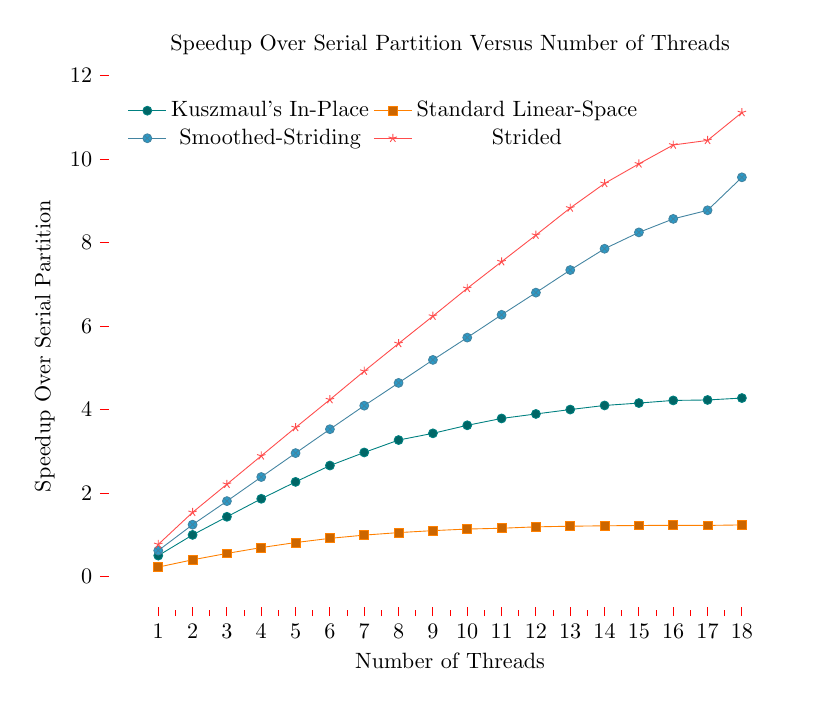
\begin{tikzpicture}[scale = .8]
\begin{axis}[
width = 5 in,
height = 4in,
title={Speedup Over Serial Partition Versus Number of Threads},
xtick pos=left,
ytick pos=left,
legend style={draw=none},
axis line style = { draw = none },
legend pos= north west,
xtick = data,
xlabel={Number of Threads},
ylabel={Speedup Over Serial Partition},
ymax = 12,
legend columns = 2,
scatter/classes=%
{a={mark=o,draw=blue}}]
%% In-Place
\addplot coordinates {( 1, 0.499048) ( 2, 0.995494) ( 3, 1.42948) ( 4, 1.86113) ( 5, 2.26614) ( 6, 2.65797) ( 7, 2.97174) ( 8, 3.26921) ( 9, 3.43004) ( 10, 3.62281) ( 11, 3.78679) ( 12, 3.89481) ( 13, 4.0002) ( 14, 4.0986) ( 15, 4.15578) ( 16, 4.2191) ( 17, 4.22999) ( 18, 4.27599) };
%% In-Place Prefix-Sum
% \addplot coordinates {( 1, 0.35092) ( 2, 0.636608) ( 3, 0.894292) ( 4, 1.11755) ( 5, 1.32674) ( 6, 1.5096) ( 7, 1.65121) ( 8, 1.77494) ( 9, 1.88432) ( 10, 1.97837) ( 11, 2.0581) ( 12, 2.11591) ( 13, 2.15699) ( 14, 2.18845) ( 15, 2.21159) ( 16, 2.21657) ( 17, 2.20736) ( 18, 2.21557) };
%% Out-of-Place
\addplot coordinates {( 1, 0.223968) ( 2, 0.398625) ( 3, 0.551717) ( 4, 0.691607) ( 5, 0.812203) ( 6, 0.912936) ( 7, 0.990429) ( 8, 1.05055) ( 9, 1.09777) ( 10, 1.13562) ( 11, 1.15517) ( 12, 1.18848) ( 13, 1.20383) ( 14, 1.21364) ( 15, 1.22103) ( 16, 1.22575) ( 17, 1.22285) ( 18, 1.23444) };
%% %% High-Span
%% \addplot coordinates {( 1, 0.796443) ( 2, 1.58021) ( 3, 2.21882) ( 4, 2.93667) ( 5, 3.32899) ( 6, 3.80217) ( 7, 4.3662) ( 8, 4.93375) ( 9, 5.09881) ( 10, 5.42822) ( 11, 5.75051) ( 12, 6.01806) ( 13, 6.37103) ( 14, 6.57999) ( 15, 6.72631) ( 16, 6.95718) ( 17, 7.06722) ( 18, 7.34442) };
%% Cache-Friendly
\addplot coordinates {( 1, 0.619888) ( 2, 1.24099) ( 3, 1.80558) ( 4, 2.38286) ( 5, 2.95654) ( 6, 3.52917) ( 7, 4.09348) ( 8, 4.63922) ( 9, 5.19034) ( 10, 5.72539) ( 11, 6.27145) ( 12, 6.80311) ( 13, 7.34442) ( 14, 7.85497) ( 15, 8.24706) ( 16, 8.57062) ( 17, 8.77723) ( 18, 9.5674) };
%% Strided
\addplot coordinates {( 1, 0.767408) ( 2, 1.5359) ( 3, 2.21084) ( 4, 2.89005) ( 5, 3.56954) ( 6, 4.2382) ( 7, 4.9214) ( 8, 5.58393) ( 9, 6.23961) ( 10, 6.90587) ( 11, 7.54451) ( 12, 8.18186) ( 13, 8.83243) ( 14, 9.4207) ( 15, 9.88984) ( 16, 10.3425) ( 17, 10.4524) ( 18, 11.1205) };
\legend{Kuszmaul's In-Place, Standard Linear-Space, Smoothed-Striding, Strided} %% Low-Space, Med-Space, High-Space, Smoothed-Striding, Strided 
\end{axis}
\end{tikzpicture}
}
\def \partitionbandwidthboundserialbaseline {3933.6}
\def \partitionbandwidthboundblocksize {64}
\def \partitionbandwidthboundnumtrials {5}
\def \partitionbandwidthboundinputsize {1073741824}
\def \partitionbandwidthboundtable {
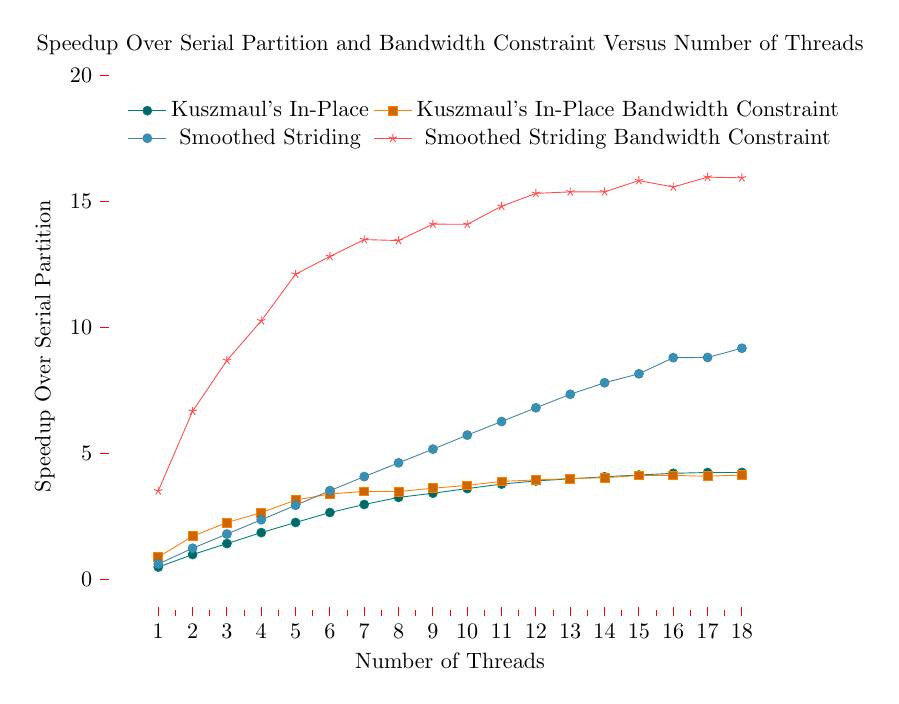
\begin{tikzpicture}[scale = .8]
\begin{axis}[
width = 5 in,
height = 4in,
title={Speedup Over Serial Partition and Bandwidth Constraint Versus Number of Threads},
xtick pos=left,
ytick pos=left,
legend style={draw=none},
axis line style = { draw = none },
legend pos= north west,
xtick = data,
xlabel={Number of Threads},
ylabel={Speedup Over Serial Partition},
ymax = 20,
legend columns = 2,
scatter/classes=%
{a={mark=o,draw=blue}}]
%% In-Place
\addplot coordinates {( 1, 0.499378) ( 2, 0.995949) ( 3, 1.4328) ( 4, 1.86816) ( 5, 2.26982) ( 6, 2.66432) ( 7, 2.98407) ( 8, 3.26602) ( 9, 3.43066) ( 10, 3.61544) ( 11, 3.79325) ( 12, 3.91949) ( 13, 4.00244) ( 14, 4.08389) ( 15, 4.15375) ( 16, 4.22151) ( 17, 4.25438) ( 18, 4.25622) };
%% Low-Space Bandwidth Bound
\addplot coordinates {(1, 0.894939)(2, 1.72634)(3, 2.26699)(4, 2.66131)(5, 3.15777)(6, 3.4024)(7, 3.50312)(8, 3.49686)(9, 3.62955)(10, 3.74294)(11, 3.90093)(12, 3.9593)(13, 4.0131)(14, 4.04714)(15, 4.13799)(16, 4.13782)(17, 4.10515)(18, 4.15355)};
%% high span
%% \addplot coordinates {( 1, 0.812828) ( 2, 1.61997) ( 3, 2.22137) ( 4, 2.95626) ( 5, 3.33582) ( 6, 3.80352) ( 7, 4.36001) ( 8, 5.10062) ( 9, 5.11521) ( 10, 5.44217) ( 11, 5.74752) ( 12, 6.07787) ( 13, 6.41278) ( 14, 6.63787) ( 15, 6.68752) ( 16, 6.79848) ( 17, 7.10549) ( 18, 7.26292) };
%% %% High-Span Bandwidth Bound
%% \addplot coordinates {(1, 1.75849)(2, 3.34185)(3, 4.35383)(4, 5.15739)(5, 5.9788)(6, 6.31621)(7, 6.76074)(8, 6.76348)(9, 6.99773)(10, 7.10173)(11, 7.39957)(12, 7.51437)(13, 7.7436)(14, 7.76191)(15, 7.89966)(16, 7.87403)(17, 7.94484)(18, 8.05483)}; %% cache friendly
\addplot coordinates {( 1, 0.62101) ( 2, 1.24639) ( 3, 1.81072) ( 4, 2.37852) ( 5, 2.95182) ( 6, 3.53233) ( 7, 4.09153) ( 8, 4.63759) ( 9, 5.18124) ( 10, 5.73746) ( 11, 6.27769) ( 12, 6.82206) ( 13, 7.35802) ( 14, 7.81717) ( 15, 8.17117) ( 16, 8.81183) ( 17, 8.81973) ( 18, 9.18636) };
%% Cache-Friendly Bandwidth Bound
\addplot coordinates {(1, 3.52223)(2, 6.68603)(3, 8.70095)(4, 10.276)(5, 12.1258)(6, 12.8292)(7, 13.4991)(8, 13.4622)(9, 14.1134)(10, 14.1066)(11, 14.8215)(12, 15.3338)(13, 15.3938)(14, 15.3942)(15, 15.8412)(16, 15.5877)(17, 15.9778)(18, 15.9519)};
\legend{Kuszmaul's In-Place, Kuszmaul's In-Place Bandwidth Constraint, Smoothed Striding, Smoothed Striding Bandwidth Constraint}
\end{axis}
\end{tikzpicture}
}

\def \CILKsortblocksize {64}
\def \CILKsortnumtrials {5}
\def \CILKsortmaxinputsize {1073741824}
\def \CILKsorttable {
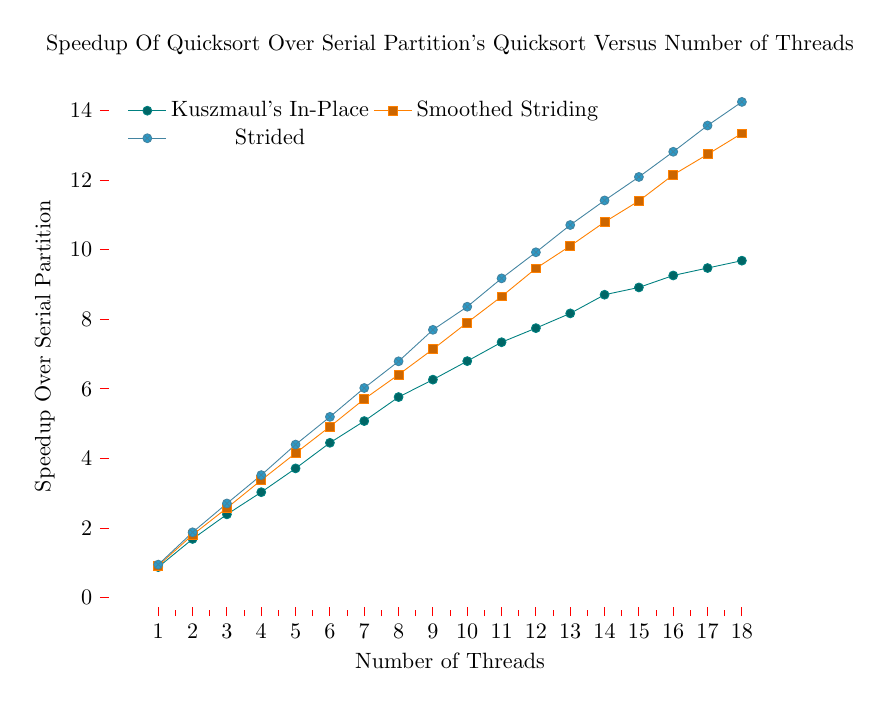
\begin{tikzpicture}[scale = .8]
\begin{axis}[
width = 5 in,
height = 4in,
title={Speedup Of Quicksort Over Serial Partition's Quicksort Versus Number of Threads},
xtick pos=left,
ytick pos=left,
legend style={draw=none},
axis line style = { draw = none },
legend pos= north west,
xtick = data,
xlabel={Number of Threads},
ylabel={Speedup Over Serial Partition},
ymax = 15,
legend columns = 2,
scatter/classes=%
{a={mark=o,draw=blue}}]
%% %% Low Space with log size 24
%% \addplot coordinates {( 1, 0.863202) ( 2, 1.63232) ( 3, 2.29705) ( 4, 2.96413) ( 5, 3.59298) ( 6, 4.1696) ( 7, 4.71085) ( 8, 5.2279) ( 9, 5.8474) ( 10, 6.4043) ( 11, 6.55736) ( 12, 7.21241) ( 13, 7.57064) ( 14, 7.99417) ( 15, 8.4679) ( 16, 8.93099) ( 17, 9.04881) ( 18, 9.60644) %% High-Span with log size 24
%% \addplot coordinates {( 1, 0.960106) ( 2, 1.88538) ( 3, 2.72075) ( 4, 3.47467) ( 5, 4.2576) ( 6, 5.08451) ( 7, 5.93339) ( 8, 6.47686) ( 9, 7.1822) ( 10, 7.57901) ( 11, 8.44704) ( 12, 8.64943) ( 13, 9.16979) ( 14, 9.04881) ( 15, 10.1464) ( 16, 9.61992) ( 17, 10.5199) ( 18, 9.38304) %% Cache Friendly with log size 24
%% \addplot coordinates {( 1, 0.900013) ( 2, 1.74752) ( 3, 2.46372) ( 4, 3.23233) ( 5, 3.90159) ( 6, 4.62508) ( 7, 5.46099) ( 8, 6.15157) ( 9, 6.85215) ( 10, 7.53736) ( 11, 8.11716) ( 12, 8.74872) ( 13, 9.70156) ( 14, 9.04881) ( 15, 11.0273) ( 16, 10.87) ( 17, 12.1829) ( 18, 12.2482) %% Strided with log size 24
%% \addplot coordinates {( 1, 0.95079) ( 2, 1.82955) ( 3, 2.63808) ( 4, 3.45716) ( 5, 4.20798) ( 6, 4.99199) ( 7, 5.78819) ( 8, 6.56364) ( 9, 7.37527) ( 10, 8.03162) ( 11, 8.89624) ( 12, 9.61992) ( 13, 9.7153) ( 14, 11.1167) ( 15, 10.9394) ( 16, 11.4891) ( 17, 13.1651) ( 18, 13.9695) };
%% %% Low Space with log size 26
%% \addplot coordinates {( 1, 0.861043) ( 2, 1.63325) ( 3, 2.3004) ( 4, 2.98343) ( 5, 3.63316) ( 6, 4.19898) ( 7, 4.82886) ( 8, 5.34581) ( 9, 5.89992) ( 10, 6.44372) ( 11, 6.94206) ( 12, 7.4672) ( 13, 7.60676) ( 14, 8.0564) ( 15, 8.64475) ( 16, 8.82709) ( 17, 8.76202) ( 18, 8.96831) %% High-Span with log size 26
%% \addplot coordinates {( 1, 0.955523) ( 2, 1.86586) ( 3, 2.6845) ( 4, 3.49224) ( 5, 4.27081) ( 6, 5.0929) ( 7, 5.83274) ( 8, 6.53586) ( 9, 7.29308) ( 10, 7.90003) ( 11, 8.63721) ( 12, 8.97915) ( 13, 9.7769) ( 14, 10.1893) ( 15, 10.5812) ( 16, 10.7887) ( 17, 10.7613) ( 18, 10.3418) %% Cache Friendly with log size 26
%% \addplot coordinates {( 1, 0.914609) ( 2, 1.73339) ( 3, 2.49178) ( 4, 3.22151) ( 5, 4.02384) ( 6, 4.70946) ( 7, 5.57239) ( 8, 6.13884) ( 9, 6.93881) ( 10, 7.59315) ( 11, 8.23047) ( 12, 8.91717) ( 13, 9.42939) ( 14, 10.1302) ( 15, 10.6801) ( 16, 10.8359) ( 17, 11.3883) ( 18, 11.3189) %% Strided with log size 26
%% \addplot coordinates {( 1, 0.946785) ( 2, 1.82922) ( 3, 2.64766) ( 4, 3.4262) ( 5, 4.2788) ( 6, 5.08245) ( 7, 5.95192) ( 8, 6.67986) ( 9, 7.44475) ( 10, 8.25563) ( 11, 8.94132) ( 12, 9.74164) ( 13, 10.4362) ( 14, 11.3621) ( 15, 11.4851) ( 16, 12.2071) ( 17, 12.6542) ( 18, 13.4993) };
%% %% Low Space with log size 28
%% \addplot coordinates {( 1, 0.862267) ( 2, 1.63941) ( 3, 2.34664) ( 4, 2.96157) ( 5, 3.64611) ( 6, 4.31258) ( 7, 4.88345) ( 8, 5.43042) ( 9, 5.87762) ( 10, 6.44029) ( 11, 7.00878) ( 12, 7.30452) ( 13, 7.83539) ( 14, 8.12956) ( 15, 8.50856) ( 16, 8.76302) ( 17, 8.98741) ( 18, 9.33821) %% High-Span with log size 28
%% \addplot coordinates {( 1, 0.939362) ( 2, 1.84744) ( 3, 2.6917) ( 4, 3.45716) ( 5, 4.29244) ( 6, 5.08279) ( 7, 5.79208) ( 8, 6.6353) ( 9, 7.2093) ( 10, 8.01682) ( 11, 8.74742) ( 12, 9.17326) ( 13, 9.7479) ( 14, 10.2979) ( 15, 11.0745) ( 16, 11.4344) ( 17, 11.4888) ( 18, 12.34) %% Cache Friendly with log size 28
%% \addplot coordinates {( 1, 0.908881) ( 2, 1.75263) ( 3, 2.51771) ( 4, 3.28228) ( 5, 4.01042) ( 6, 4.74982) ( 7, 5.54834) ( 8, 6.2393) ( 9, 6.98884) ( 10, 7.70125) ( 11, 8.41219) ( 12, 9.06778) ( 13, 9.67555) ( 14, 10.3505) ( 15, 11.0125) ( 16, 11.4744) ( 17, 12.1533) ( 18, 12.4095) %% Strided with log size 28
%% \addplot coordinates {( 1, 0.942529) ( 2, 1.82563) ( 3, 2.6044) ( 4, 3.46053) ( 5, 4.25683) ( 6, 5.12315) ( 7, 5.88602) ( 8, 6.70811) ( 9, 7.43113) ( 10, 8.17952) ( 11, 8.96974) ( 12, 9.68435) ( 13, 10.4214) ( 14, 10.9587) ( 15, 11.71) ( 16, 12.2949) ( 17, 12.9046) ( 18, 13.3107) };
%% Low Space with log size 30
\addplot coordinates {( 1, 0.87864) ( 2, 1.68661) ( 3, 2.39404) ( 4, 3.03172) ( 5, 3.71549) ( 6, 4.45118) ( 7, 5.07595) ( 8, 5.76618) ( 9, 6.26716) ( 10, 6.79929) ( 11, 7.34223) ( 12, 7.74736) ( 13, 8.17148) ( 14, 8.70784) ( 15, 8.91736) ( 16, 9.26139) ( 17, 9.47532) ( 18, 9.68665)}; %% High-Span with log size 30
%% \addplot coordinates {( 1, 0.96225) ( 2, 1.879) ( 3, 2.71741) ( 4, 3.56118) ( 5, 4.44821) ( 6, 5.29223) ( 7, 5.97895) ( 8, 6.76091) ( 9, 7.59373) ( 10, 8.37912) ( 11, 9.01587) ( 12, 9.58729) ( 13, 10.1906) ( 14, 10.881) ( 15, 11.4166) ( 16, 12.026) ( 17, 12.3279) ( 18, 12.6408)}; %% Cache Friendly with log size 30
\addplot coordinates {( 1, 0.921182) ( 2, 1.80562) ( 3, 2.57745) ( 4, 3.37831) ( 5, 4.15358) ( 6, 4.91613) ( 7, 5.7093) ( 8, 6.41041) ( 9, 7.14098) ( 10, 7.907) ( 11, 8.6573) ( 12, 9.46479) ( 13, 10.1098) ( 14, 10.7975) ( 15, 11.4046) ( 16, 12.1549) ( 17, 12.7427) ( 18, 13.346)}; %% Strided with log size 30
\addplot coordinates {( 1, 0.949951) ( 2, 1.87888) ( 3, 2.70758) ( 4, 3.52248) ( 5, 4.40049) ( 6, 5.19675) ( 7, 6.02708) ( 8, 6.79362) ( 9, 7.69896) ( 10, 8.36354) ( 11, 9.17828) ( 12, 9.92823) ( 13, 10.7114) ( 14, 11.4187) ( 15, 12.0935) ( 16, 12.8171) ( 17, 13.5719) ( 18, 14.2507) };
\legend{Kuszmaul's In-Place, Smoothed Striding, Strided}
\end{axis}
\end{tikzpicture}
}

%% Bandwith results without numactl:
%% \def \partitionbandwidthboundserialbaseline {3832}
%% \def \partitionbandwidthboundblocksize {64}
%% \def \partitionbandwidthboundnumtrials {5}
%% \def \partitionbandwidthboundinputsize {1073741824}
%% \def \partitionbandwidthboundtable {
%% \begin{tikzpicture}[scale = .8]
%% \begin{axis}[
%% width = 5 in,
%% height = 4in,
%% title={Speedup Versus Number of Threads},
%% xtick pos=left,
%% ytick pos=left,
%% legend style={draw=none},
%% axis line style = { draw = none },
%% legend pos= north west,
%% xtick = data,
%% xlabel={Number of Threads},
%% ylabel={Speedup Over Serial Partition},
%% ymax = 4,
%% legend columns = 2,
%% scatter/classes=%
%% {a={mark=o,draw=blue}}]
%% %% In-Place
%% \addplot coordinates {( 1, 0.504928) ( 2, 0.744917) ( 3, 1.27793) ( 4, 1.62967) ( 5, 1.91677) ( 6, 2.3244) ( 7, 2.47865) ( 8, 2.58186) ( 9, 2.68573) ( 10, 2.78448) ( 11, 2.7756) ( 12, 2.85077) ( 13, 2.86826) ( 14, 2.91407) ( 15, 2.90479) ( 16, 2.94769) ( 17, 2.95497) ( 18, 2.94588) };
%% %% Low-Space Bandwidth Bound
%% \addplot coordinates {(1, 1.05385)(2, 1.63936)(3, 1.81183)(4, 2.05614)(5, 2.39067)(6, 2.5237)(7, 2.40513)(8, 2.55015)(9, 2.58884)(10, 2.57444)(11, 2.69167)(12, 2.66946)(13, 2.64859)(14, 2.68175)(15, 2.66023)(16, 2.69318)(17, 2.68783)(18, 2.72913)};
%% %% high span
%% \addplot coordinates {( 1, 0.816814) ( 2, 1.47691) ( 3, 1.98529) ( 4, 2.63875) ( 5, 3.01305) ( 6, 3.40441) ( 7, 3.68887) ( 8, 3.97345) ( 9, 4.14181) ( 10, 4.27297) ( 11, 4.46724) ( 12, 4.45271) ( 13, 4.45271) ( 14, 4.62355) ( 15, 4.60024) ( 16, 4.70184) ( 17, 4.55431) ( 18, 4.71225) };
%% %% High-Span Bandwidth Bound
%% \addplot coordinates {(1, 2.03744)(2, 3.14521)(3, 3.47353)(4, 3.91661)(5, 4.536)(6, 4.70395)(7, 4.47075)(8, 4.76355)(9, 4.86065)(10, 4.68934)(11, 4.86418)(12, 4.98468)(13, 4.9239)(14, 4.99117)(15, 4.94174)(16, 4.98761)(17, 4.96382)(18, 5.00564)%% cache friendly
%% \addplot coordinates {( 1, 0.621291) ( 2, 1.06581) ( 3, 1.76541) ( 4, 2.28204) ( 5, 2.8838) ( 6, 3.49253) ( 7, 4.04561) ( 8, 4.56843) ( 9, 4.97921) ( 10, 5.6089) ( 11, 5.8791) ( 12, 6.26963) ( 13, 6.8331) ( 14, 6.87971) ( 15, 7.15459) ( 16, 7.38343) ( 17, 8.25151) ( 18, 8.35587) };
%% %% Cache-Friendly Bandwidth Bound
%% \addplot coordinates {(1, 4.06363)(2, 6.29023)(3, 6.9299)(4, 7.88794)(5, 9.08502)(6, 9.329)(7, 9.45987)(8, 9.53406)(9, 9.91163)(10, 9.90729)(11, 9.70433)(12, 10.1146)(13, 9.9126)(14, 9.85886)(15, 9.86993)(16, 10.0183)(17, 10.0765)(18, 9.99261)};
%% \legend{Low-Space, Low-Space Bandwidth Constraint, Two-Layer, Two-Layer Bandwidth Constraint}
%% \end{axis}
%% \end{tikzpicture}
%% }

%\def \CILKserialbaseline {1}
\def \CILKblocksize {64}
\def \CILKnumtrials {5}
\def \CILKinputsize {262144}
\def \CILKtable {
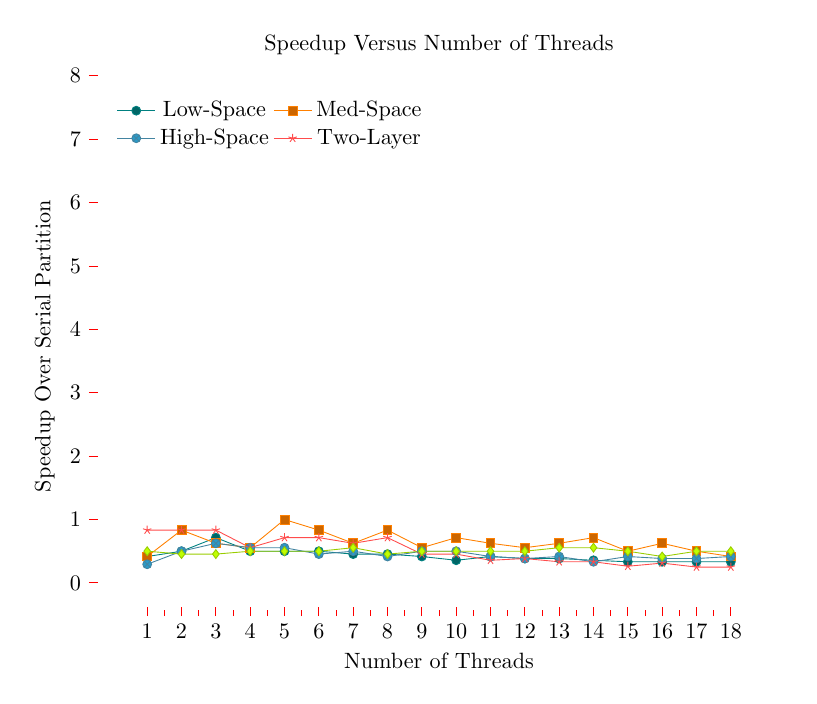
\begin{tikzpicture}[scale = .8]
\begin{axis}[
width = 5 in,
height = 4in,
title={Speedup Versus Number of Threads},
xtick pos=left,
ytick pos=left,
legend style={draw=none},
axis line style = { draw = none },
legend pos= north west,
xtick = data,
xlabel={Number of Threads},
ylabel={Speedup Over Serial Partition},
ymax = 8,
legend columns = 2,
scatter/classes=%
{a={mark=o,draw=blue}}]
%% In-Place
\addplot coordinates {( 1, 0.416667) ( 2, 0.5) ( 3, 0.714286) ( 4, 0.5) ( 5, 0.5) ( 6, 0.5) ( 7, 0.454545) ( 8, 0.454545) ( 9, 0.416667) ( 10, 0.357143) ( 11, 0.416667) ( 12, 0.384615) ( 13, 0.384615) ( 14, 0.357143) ( 15, 0.333333) ( 16, 0.333333) ( 17, 0.333333) ( 18, 0.333333) };
%% In-Place Prefix-Sum
\addplot coordinates {( 1, 0.416667) ( 2, 0.833333) ( 3, 0.625) ( 4, 0.555556) ( 5, 1) ( 6, 0.833333) ( 7, 0.625) ( 8, 0.833333) ( 9, 0.555556) ( 10, 0.714286) ( 11, 0.625) ( 12, 0.555556) ( 13, 0.625) ( 14, 0.714286) ( 15, 0.5) ( 16, 0.625) ( 17, 0.5) ( 18, 0.416667) };
%% Out-of-Place
\addplot coordinates {( 1, 0.294118) ( 2, 0.5) ( 3, 0.625) ( 4, 0.555556) ( 5, 0.555556) ( 6, 0.454545) ( 7, 0.5) ( 8, 0.416667) ( 9, 0.5) ( 10, 0.5) ( 11, 0.416667) ( 12, 0.384615) ( 13, 0.416667) ( 14, 0.333333) ( 15, 0.416667) ( 16, 0.384615) ( 17, 0.384615) ( 18, 0.416667) };
%% High-Span
\addplot coordinates {( 1, 0.833333) ( 2, 0.833333) ( 3, 0.833333) ( 4, 0.555556) ( 5, 0.714286) ( 6, 0.714286) ( 7, 0.625) ( 8, 0.714286) ( 9, 0.454545) ( 10, 0.454545) ( 11, 0.357143) ( 12, 0.384615) ( 13, 0.333333) ( 14, 0.333333) ( 15, 0.263158) ( 16, 0.3125) ( 17, 0.25) ( 18, 0.25) };
%% Cache-Friendly
\addplot coordinates {( 1, 0.5) ( 2, 0.454545) ( 3, 0.454545) ( 4, 0.5) ( 5, 0.5) ( 6, 0.5) ( 7, 0.555556) ( 8, 0.454545) ( 9, 0.5) ( 10, 0.5) ( 11, 0.5) ( 12, 0.5) ( 13, 0.555556) ( 14, 0.555556) ( 15, 0.5) ( 16, 0.416667) ( 17, 0.5) ( 18, 0.5) };
\legend{Low-Space, Med-Space, High-Space, Two-Layer}
\end{axis}
\end{tikzpicture}
}
\def \cilktwoblocksizetwo {64}
\def \cilktwonumtrialstwo {5}
\def \cilktwonumcorestwo {18}
\def \cilktwoinputsizetwo {262144}
\def \cilktwotabletwo {
\begin{tikzpicture}[scale = .8]
\begin{axis}[
width = 5 in,
height = 4in,
title={Speedup Versus Input Size},
xtick pos=left,
ytick pos=left,
legend style={draw=none},
axis line style = { draw = none },
legend pos= north west,
xtick = data,
xlabel={Log Input Size},
ylabel={Speedup Over Serial Partition},
ymax = 5,
ymin = 0,
legend columns = 2,
scatter/classes=%
{a={mark=o,draw=blue}}]
%% Serial Baseline
%% baselines in ms: \addplot coordinates {};
%% In-Place
\addplot coordinates {};
%% In-Place Prefix-Sum
\addplot coordinates {};
%% Out-of-Place
\addplot coordinates {};
%% High-Span
\addplot coordinates {};
%% Cache-Friendly
\addplot coordinates {};
\legend{Low-Space, Med-Space, High-Space, Two-Layer}
\end{axis}
\end{tikzpicture}
}
\def \CILKsortblocksize {64}
\def \CILKsortnumtrials {5}
\def \CILKsortmaxinputsize {262144}
\def \CILKsorttable {
\begin{tikzpicture}[scale = .8]
\begin{axis}[
width = 5 in,
height = 4in,
title={Speedup Versus Number of Threads},
xtick pos=left,
ytick pos=left,
legend style={draw=none},
axis line style = { draw = none },
legend pos= north west,
xtick = data,
xlabel={Number of Threads},
ylabel={Speedup Over Serial Partition},
ymax = 6,
legend columns = 2,
scatter/classes=%
{a={mark=o,draw=blue}}]
\legend{ Low-Space 24, Low-Space 26, Low-Space 28, Two-Layer 24, Two-Layer 26, Two-Layer 28}
\end{axis}
\end{tikzpicture}
}
\def \partitionbandwidthboundserialbaseline {1.4}
\def \partitionbandwidthboundblocksize {64}
\def \partitionbandwidthboundnumtrials {5}
\def \partitionbandwidthboundinputsize {262144}
\def \partitionbandwidthboundtable {
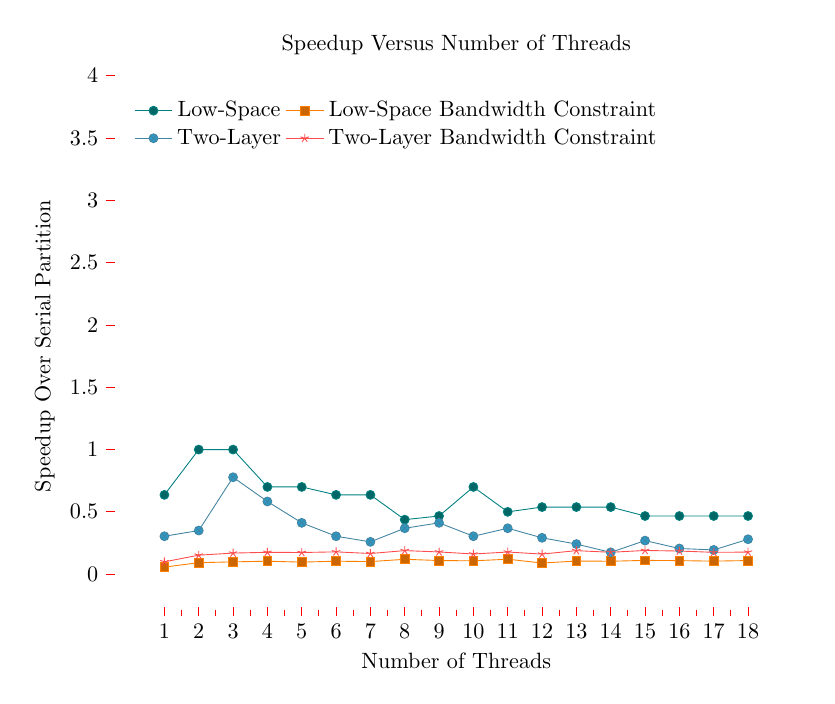
\begin{tikzpicture}[scale = .8]
\begin{axis}[
width = 5 in,
height = 4in,
title={Speedup Versus Number of Threads},
xtick pos=left,
ytick pos=left,
legend style={draw=none},
axis line style = { draw = none },
legend pos= north west,
xtick = data,
xlabel={Number of Threads},
ylabel={Speedup Over Serial Partition},
ymax = 4,
legend columns = 2,
scatter/classes=%
{a={mark=o,draw=blue}}]
%% In-Place
\addplot coordinates {( 1, 0.636364) ( 2, 1) ( 3, 1) ( 4, 0.7) ( 5, 0.7) ( 6, 0.636364) ( 7, 0.636364) ( 8, 0.4375) ( 9, 0.466667) ( 10, 0.7) ( 11, 0.5) ( 12, 0.538462) ( 13, 0.538462) ( 14, 0.538462) ( 15, 0.466667) ( 16, 0.466667) ( 17, 0.466667) ( 18, 0.466667) };
%% Low-Space Bandwidth Bound
\addplot coordinates {(1, 0.0566392)(2, 0.0918376)(3, 0.0985994)(4, 0.103927)(5, 0.0965002)(6, 0.103986)(7, 0.100812)(8, 0.119203)(9, 0.109285)(10, 0.106923)(11, 0.119862)(12, 0.0891909)(13, 0.105142)(14, 0.103583)(15, 0.110553)(16, 0.108612)(17, 0.104464)(18, 0.109112)};
%% high span
\addplot coordinates {( 1, 0.304348) ( 2, 0.35) ( 3, 0.777778) ( 4, 0.583333) ( 5, 0.411765) ( 6, 0.304348) ( 7, 0.259259) ( 8, 0.368421) ( 9, 0.411765) ( 10, 0.304348) ( 11, 0.368421) ( 12, 0.291667) ( 13, 0.241379) ( 14, 0.175) ( 15, 0.269231) ( 16, 0.205882) ( 17, 0.194444) ( 18, 0.28) };
%% High-Span Bandwidth Bound
\addplot coordinates {(1, 0.0989274)(2, 0.152213)(3, 0.16911)(4, 0.175354)(5, 0.173704)(6, 0.178873)(7, 0.165707)(8, 0.188904)(9, 0.178216)(10, 0.161825)(11, 0.177553)(12, 0.161085)(13, 0.188701)(14, 0.175466)(15, 0.190048)(16, 0.185474)(17, 0.175112)(18, 0.176937)};
\legend{Low-Space, Low-Space Bandwidth Constraint, Two-Layer, Two-Layer Bandwidth Constraint}
\end{axis}
\end{tikzpicture}
}
 % ALEK ALEK ALEK
\def \serialnumtrials {5}
\def \serialblocksize {64}
\def \serialtable {
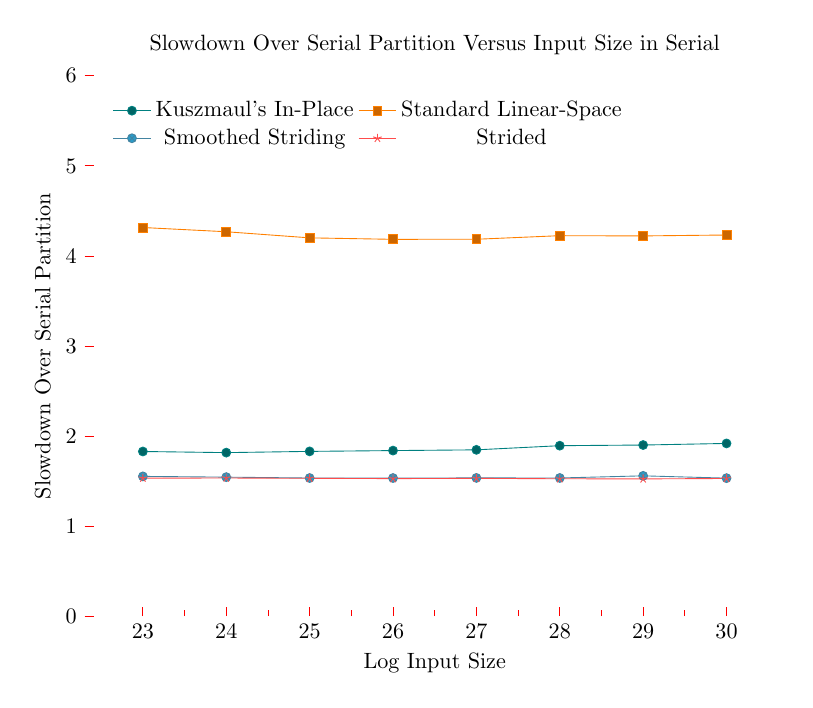
\begin{tikzpicture}[scale = .8]
\begin{axis}[
width = 5 in,
height = 4in,
title={Slowdown Over Serial Partition Versus Input Size in Serial},
xtick pos=left,
ytick pos=left,
ymax = 6,
ymin = 0,
legend style={draw=none},
axis line style = { draw = none },
legend pos= north west,
xtick = data,
xlabel={Log Input Size},
ylabel={Slowdown Over Serial Partition},
legend columns = 2,
scatter/classes=%
{a={mark=o,draw=blue}}]
%% Serial Baseline
%% baselines in ms: \addplot coordinates {( 23, 30.4 ) ( 24, 61 ) ( 25, 122.4 ) ( 26, 244.8 ) ( 27, 489.6 ) ( 28, 979.6 ) ( 29, 1963.4 ) ( 30, 3922.6 ) };
%% In-Place
\addplot coordinates {( 23, 1.82895) ( 24, 1.81639) ( 25, 1.83007) ( 26, 1.83905) ( 27, 1.84722) ( 28, 1.89343) ( 29, 1.90068) ( 30, 1.91837) };
%% In-Place Prefix-Sum
% \addplot coordinates {( 23, 2.75658) ( 24, 2.71803) ( 25, 2.68137) ( 26, 2.67157) ( 27, 2.67443) ( 28, 2.70131) ( 29, 2.70551) ( 30, 2.71713) };
%% Out-of-Place
\addplot coordinates {( 23, 4.31579) ( 24, 4.26885) ( 25, 4.20098) ( 26, 4.18464) ( 27, 4.18546) ( 28, 4.22519) ( 29, 4.22257) ( 30, 4.23265) };
%% %% High-Span
%% \addplot coordinates {( 23, 1.23684) ( 24, 1.23934) ( 25, 1.24346) ( 26, 1.24428) ( 27, 1.24632) ( 28, 1.24602) ( 29, 1.24417) ( 30, 1.2456) };
%% Cache-Friendly
\addplot coordinates {( 23, 1.55263) ( 24, 1.54426) ( 25, 1.53431) ( 26, 1.53431) ( 27, 1.53554) ( 28, 1.53491) ( 29, 1.55852) ( 30, 1.53317) };
%% Strided
\addplot coordinates {( 23, 1.53289) ( 24, 1.53443) ( 25, 1.53105) ( 26, 1.52778) ( 27, 1.53064) ( 28, 1.52613) ( 29, 1.5246) ( 30, 1.52919) };
\legend{Kuszmaul's In-Place, Standard Linear-Space, Smoothed Striding, Strided} % Low-Space, Med-Space, High-Space, Smoothed Striding, Strided
\end{axis}
\end{tikzpicture}
}
%% \def \serialnumtrials {5}
%% \def \serialblocksize {64}
%% \def \serialtable {
%% \begin{tikzpicture}[scale = .8]
%% \begin{axis}[
%% width = 5 in,
%% height = 4in,
%% title={Slowdown Versus Input Size in Serial},
%% xtick pos=left,
%% ytick pos=left,
%% ymax = 5,
%% ymin = 0,
%% legend style={draw=none},
%% axis line style = { draw = none },
%% legend pos= north west,
%% xtick = data,
%% xlabel={Log Input Size},
%% ylabel={Slowdown Over Serial Partition},
%% legend columns = 2,
%% scatter/classes=%
%% {a={mark=o,draw=blue}}]
%% %% Serial Baseline
%% %% baselines in ms: \addplot coordinates {( 23, 30.4 ) ( 24, 61 ) ( 25, 122.4 ) ( 26, 244.8 ) ( 27, 489.6 ) ( 28, 979.6 ) ( 29, 1963.4 ) ( 30, 3922.6 ) };
%% %% In-Place
%% \addplot coordinates {( 23, 1.82895) ( 24, 1.81639) ( 25, 1.83007) ( 26, 1.83905) ( 27, 1.84722) ( 28, 1.89343) ( 29, 1.90068) ( 30, 1.91837) };
%% %% In-Place Prefix-Sum
%% \addplot coordinates {( 23, 2.75658) ( 24, 2.71803) ( 25, 2.68137) ( 26, 2.67157) ( 27, 2.67443) ( 28, 2.70131) ( 29, 2.70551) ( 30, 2.71713) };
%% %% Out-of-Place
%% \addplot coordinates {( 23, 4.31579) ( 24, 4.26885) ( 25, 4.20098) ( 26, 4.18464) ( 27, 4.18546) ( 28, 4.22519) ( 29, 4.22257) ( 30, 4.23265) };
%% %% High-Span
%% \addplot coordinates {( 23, 1.23684) ( 24, 1.23934) ( 25, 1.24346) ( 26, 1.24428) ( 27, 1.24632) ( 28, 1.24602) ( 29, 1.24417) ( 30, 1.2456) };
%% %% Cache-Friendly
%% \addplot coordinates {( 23, 1.55263) ( 24, 1.54426) ( 25, 1.53431) ( 26, 1.53431) ( 27, 1.53554) ( 28, 1.53491) ( 29, 1.55852) ( 30, 1.53317) };
%% %% Strided
%% \addplot coordinates {( 23, 1.53289) ( 24, 1.53443) ( 25, 1.53105) ( 26, 1.52778) ( 27, 1.53064) ( 28, 1.52613) ( 29, 1.5246) ( 30, 1.52919) };
%% \legend{Low-Space, Med-Space, High-Space, Two-Layer, Cache-Friendly, Strided}
%% \end{axis}
%% \end{tikzpicture}
%% }
%% \def \serialnumtrials {1}
%% \def \serialblocksize {64}
%% \def \serialtable {
%% \begin{tikzpicture}[scale = .8]
%% \begin{axis}[
%% title={Slowdown Versus Input Size in Serial},
%% width = 5in, %%!!!!
%% height = 4in,
%% xtick pos=left,
%% ytick pos=left,
%% ymax = 5, %% !!!
%% ymin = 0,
%% legend style={draw=none},
%% axis line style = { draw = none },
%% legend pos= north west,
%% xtick = data,
%% xlabel={Log Input Size},
%% ylabel={Slowdown Over Serial Partition},
%% legend columns = 2,
%% scatter/classes=%
%% {a={mark=o,draw=blue}}]
%% %% Serial Baseline%% baselines in ms: \addplot coordinates {( 23, 30.4 ) ( 24, 60.8 ) ( 25, 121.4 ) ( 26, 243.8 ) ( 27, 487.4 ) ( 28, 975.8 ) ( 29, 1952.2 ) ( 30, 3902 ) };
%% %% In-Place
%% \addplot coordinates {( 23, 1.79605) ( 24, 1.82237) ( 25, 1.84185) ( 26, 1.84249) ( 27, 1.87033) ( 28, 1.90838) ( 29, 1.90687) ( 30, 1.91579) };
%% %% In-Place Prefix-Sum
%% \addplot coordinates {( 23, 2.58553) ( 24, 2.57237) ( 25, 2.57661) ( 26, 2.56932) ( 27, 2.56422) ( 28, 2.59459) ( 29, 2.60834) ( 30, 2.61107) };
%% %% Out-of-Place
%% \addplot coordinates {( 23, 3.98684) ( 24, 3.96711) ( 25, 3.96705) ( 26, 3.96308) ( 27, 3.98195) ( 28, 4.01537) ( 29, 4.03401) ( 30, 4.06079) };
%% %% High-Span
%% \addplot coordinates {( 23, 1.21053) ( 24, 1.23355) ( 25, 1.23558) ( 26, 1.23298) ( 27, 1.23677) ( 28, 1.24124) ( 29, 1.24096) ( 30, 1.23931) };
%% \legend{Low-Space, Med-Space, High-Space, Two-Layer} %% Two-layer instead of high-span everywhere
%% \end{axis}
%% \end{tikzpicture}
%% }
%% %% Speedup on 18 threads in table of size 268435456
%% \def \serialsortspeedup {0.780189}


\newcommand{\dec}{\operatorname{dec}}
\newcommand{\github}{\url{github.com/williamkuszmaul/Parallel-Partition}}
\newcommand{\defn}[1]       {{\textit{\textbf{\boldmath #1}}}}
\renewcommand{\paragraph}[1]{\vspace{0.09in}\noindent{\bf \boldmath #1.}} 
\usepackage{amsmath}
\usepackage{amssymb}
\usepackage{amsthm}
\usepackage{todonotes}

\newtheorem{thm}{Theorem}[section]
\newtheorem{lem}[thm]{Lemma}
\newtheorem{prop}[thm]{Proposition}
\newtheorem{clm}[thm]{Claim}
\newtheorem{cor}[thm]{Corollary}
\newtheorem{conj}[thm]{Conjecture}
\theoremstyle{remark}
\newtheorem{rem}[thm]{Remark}
\newtheorem{ex}[thm]{Example}

\newtheorem{theorem}{Theorem}[section]
\newtheorem{definition}[thm]{Definition}
\newtheorem{lemma}[thm]{Lemma}
\newtheorem{proposition}[thm]{Proposition}
\newtheorem{claim}[thm]{Claim}
\newtheorem{corollary}[thm]{Corollary}
\newtheorem{conjecture}[thm]{Conjecture}
\theoremstyle{remark}
\newtheorem{remark}[thm]{Remark}
\newtheorem{example}[thm]{Example}
\newtheorem{observation}[thm]{Observation}

\usepackage{hyperref}



\begin{document}
\title{Simple and Space-Efficient Parallel-Partition Algorithms using Exclusive-Read-and-Write Memory}
\subtitle{}

\author{William Kuszmaul}
\authornote{Supported by a Hertz Fellowship and a NSF GRFP Fellowship}
\affiliation{%
  \institution{Massachusetts Institute of Technology}
}
\email{kuszmaul@mit.edu}


% The default list of authors is too long for headers.
\renewcommand{\shortauthors}{William Kuszmaul}


\begin{abstract}
We present a simple in-place algorithm for parallel partition that has
work $O(n)$ and span $O(\log n \cdot \log \log n)$. The algorithm uses
only exclusive read/write shared variables, and can be implemented
using parallel-for-loops without any additional concurrency
considerations (i.e., the algorithm is in the EREW PRAM model). As an
immediate consequence, we also get a simple in-place quicksort
algorithm with work $O(n \log n)$ and span $O(\log^2 n \log \log n)$.

Using our algorithmic techniques, we implement an (almost) in-place
parallel partition. In addition to achieving much better memory
utilization, the algorithm leverages its improved cache behavior to
achieve a speedup over its out-of-place counterpart.

We also present an alternative in-place parallel-partition algorithm
with a larger span of $O(\sqrt{n \log n})$, but which is designed to
have very small overhead. We show that when the algorithm
is tuned appropriately, and given a large enough input to achieve high
parallelism, the algorithm can be made to outperform is lower-span
peers.


\end{abstract}

%
% The code below should be generated by the tool at
% http://dl.acm.org/ccs.cfm
% Please copy and paste the code instead of the example below.
%
\begin{CCSXML}
<ccs2012>
<concept>
<concept_id>10003752.10003809.10010170.10010171</concept_id>
<concept_desc>Theory of computation~Shared memory algorithms</concept_desc>
<concept_significance>500</concept_significance>
</concept>
</ccs2012>
\end{CCSXML}

\ccsdesc[500]{Theory of computation~Shared memory algorithms}

\keywords{Parallel Partition, EREW PRAM, in-place algorithms}


\maketitle





 

\section{Introduction}

A \defn{parallel partition} operation rearranges the elements in an
array so that the elements satisfying a particular \defn{pivot
  property} appear first. In addition to playing a central role in
parallel quicksort, the parallel partition operation is used as a
primitive throughout parallel algorithms.\footnote{In several
  well-known textbooks and surveys on parallel algorithms
  \cite{AcarBl16,Blelloch96}, for example, parallel partitions are
  implicitly used extensively to perform what are referred to as
  \emph{filter} operations.}

A parallel algorithm can be measured by its \defn{work}, the time
needed to execute in serial, and its \defn{span}, the time to execute
on infinitely many processors. There is a well-known algorithm for
parallel partition on arrays of size $n$ with work $O(n)$ and span
$O(\log n)$ \cite{Blelloch96,AcarBl16}. Moreover, the algorithm uses
only exclusive read/write shared memory variables (i.e., it is an
\defn{EREW} algorithm). This eliminates the need for concurrency
mechanisms such as locks and atomic variables, and ensures good
behavior even if the time to access a location is a function of the
number of threads trying to access it (or its cache line)
concurrently. EREW algorithms also have the advantage that their
behavior is internally deterministic, meaning that
the behavior of the algorithm will not differ from run to run, which
makes test coverage, debugging, and reasoning about performance
substantially easier \cite{BlellochFi12}.

The parallel-partition algorithm suffers from using a large amount of
auxiliary memory, however. Whereas the serial algorithm is typically
implemented in place, the parallel algorithm relies on the use of two
auxiliary arrays of size $n$. To the best of our knowledge, the only
known linear-work and $\operatorname{polylog}(n)$-span algorithms for
parallel partition that are in-place require the use of atomic
operations (e.g, fetch-and-add)
\cite{HeidelbergerNo90,AxtmannWi17,TsigasZh03}.

An algorithm's memory efficiency can be critical on large inputs. The
memory consumption of an algorithm determines the largest problem size
that can be executed in memory. Many external memory algorithms (i.e.,
algorithms for problems too large to fit in memory) perform large
subproblems in memory; the size of these subproblems is again
bottlenecked by the algorithm's memory-overhead \cite{Vitter08}. In
multi-user systems, memory efficiency is also important on small
inputs, since processes with larger memory-footprints can hog the
cache, slowing down other processes. 

For sorting algorithms, in particular, special attention to memory
efficiency is often given. This is because (a) a user calling the sort
function may already be using almost all of the memory in the system;
and (b) sorting algorithms, and especially parallel sorting
algorithms, are often bottlenecked by memory bandwidth.

In the context of parallel algorithms, however, the most practically
efficient sorting algorithms fail to run in place, at least without
the additional use of atomic-fetch-and-add variables
\cite{HeidelbergerNo90, AxtmannWi17, TsigasZh03}, or the loss of
theoretical guarantees on parallelism \cite{FrancisPa92}. Parallel
merge sort \cite{Hagerup89} was made in-place by Katajainen
\cite{Katajainen93}, but has proven too sophisticated for practical
applications. Bitonic sort \cite{BlellochLe98} is naturally in-place,
and can be practical in certain applications on super computers, but
suffers in general from requiring work $\Theta(n \log^2 n)$ rather
than $O(n \log n)$. Parallel quicksort, on the other hand, despite the
many efforts to optimize it \cite{HeidelbergerNo90, AxtmannWi17,
  TsigasZh03, FrancisPa92, Frias08}, has eluded any in-place EREW (or
even CREW) algorithms due to its reliance on parallel
partition.\footnote{In a \defn{CREW} algorithm, reads may be
  concurrent, but writes may not. CREW stands for
  \emph{concurrent-read exclusive-write}.}


\paragraph{Results}
We present a simple in-place algorithm for parallel partition that has
work $O(n)$ and span $O(\log n \cdot \log \log n)$. The algorithm uses
only exclusive read/write shared variables, and can be implemented
using parallel-for-loops without any additional concurrency
considerations. As an immediate consequence, we also get a simple
in-place quicksort algorithm with work $O(n \log n)$ and span
$O(\log^2 n \log \log n)$.

Using our algorithmic techniques, we implement and optimize a
space-efficient parallel partition. Because the in-place algorithm
eliminates the use of large auxiliary arrays, the algorithm is able to
achieve a significant reduction in cache misses over its out-of-place
counterpart, resulting in performance improvements both in serial and
in parallel.

We also present an alternative in-place parallel-partition algorithm
with a larger span of $O(\sqrt{n \log n})$, but which is designed to
have very small engineering overhead. On a single core, the algorithm
performs within 25\% of the serial GNU Libc quicksort partition
algorithm. We show that when the algorithm is tuned appropriately, and
given a large enough input to achieve high parallelism, the algorithm
can be made to outperform is lower-span peers. The low-span
algorithms, on the other hand, ensure good scaling with less
sensitivity to the number of cores and the input size.


\section{Preliminaries}\label{secprelim}

We begin by describing the the parallelism and memory model used in
the paper, and by presenting background on parallel partition.

\paragraph{Workflow Model} We consider a language-based model of parallelism in which algorithms may achieve parallelism
through the use of \defn{parallel-for-loops}, though our algorithm
also works in the less restrictive PRAM model
\cite{Blelloch96,AcarBl16}.  A parallel-for-loop is given a range $R
\in \mathbb{N}$, a constant number of arguments $\arg_1, \arg_2,
\ldots, \arg_c$, and a body of code. For each $i \in \{1, \ldots,
R\}$, the loop launches a thread that is given loop-counter $i$ and
local copies of the arguments $\arg_1, \arg_2, \ldots, \arg_c$. The
threads then perform the body of the loop.\footnote{Note that
  parallel-for-loops also implicitly allow for the implementation of
  parallel recursion by placing recursive function calls in the body
  of the parallel-for-loop.}

A parallel algorithm may be run on an arbitrary number $p$ of
processors. The algorithm itself is oblivious to $p$, however, leaving
the assignment of threads to processors up to a scheduler.

The \defn{work} $T_1$ of an algorithm is the time that the algorithm
would require to execute on a single processor. The \defn{span}
$T_\infty$ of an algorithm is the time to execute on infinitely many
processors. The scheduler is assumed to contribute no overhead to the
span. In particular, if the body of a
parallel-for-loop has span $s$, then the full parallel loop has span
$s + O(1)$ \cite{Blelloch96,AcarBl16}.

The work $T_1$ and span $T_\infty$ can be used to quantify the time $T_p$
that an algorithm requires to execute on $p$ processors using a greedy
online scheduler. If the scheduler is assumed to contribute no
overhead, then Brent's Theorem \cite{Brent74} states that for any
$p$,
$$T_1 / p \le T_p \le T_1 / p + T_\infty.$$

The work-stealing algorithms used in the Cilk extension of C/C++ realize
the guarantee offered by Brent's Theorem within a constant factor
\cite{BlumofeJo96,BlumofeLe99}, with the added caveat that parallel-for-loops typically induce an additional additive overhead of $O(\log
R)$.

\paragraph{Memory Model} Memory is \defn{exclusive-read} and \defn{exclusive-write}. That is, no two threads are ever permitted to attempt to read or write to the same variable concurrently. The exclusive-read exclusive-write memory model is sometime referred to as the \defn{EREW model} (see, e.g., \cite{Hagerup89}).

In an \defn{in-place} algorithm, each thread is given $O(\log n)$
memory upon creation that is deallocated when the thread dies. This
memory can be shared with the thread's children. The depth of the
parent-child tree is not permitted to exceed $O(\log n)$.\footnote{The
  algorithm in this paper satisfies a slightly stronger property that
  the total memory being used is never more than $O(\log n) \cdot p$,
  where $p$ is an upper-bound on the number of worker threads.}

\paragraph{The Parallel Partition Problem}
The parallel partition problem takes an input array $A$ of size $n$,
and a \defn{decider function} $\dec$ that determines for each element
$a[i] \in A$ whether or not $A[i]$ is a \defn{predecessor} or a
\defn{successor}. That is, $\dec(A[i]) = 1$ if $A[i]$ is a
predecessor, and $\dec(A[i]) = 0$ if $A[i]$ is a successor. The
behavior of the parallel partition is to reorder the elements in the
array $A$ so that the predecessors appear before the successors.


\paragraph{The (Standard) Linear-Space Parallel Partition} The linear-space implementation of parallel partition consists of two phases \cite{Blelloch96,AcarBl16}:

\noindent\emph{The Parallel-Prefix Phase: }In this phase, the algorithm
constructs an array $B$ whose $i$-th element $B[i] = \sum_{j = 1}^i
\dec(A[i])$ is the number of predecessors in the first $i$ elements of
$A$. The transformation from $A$ to $B$ is called a \defn{parallel
  prefix sum} and can be performed with $O(n)$ work and $O(\log n)$
span using a simple recursive algorithm: (1) First construct an array
$A'$ of size $n / 2$ with $A'[i] = A[2i - 1] + A[2i]$; (2)
Recursively construct a parallel prefix sum $B'$ of $A'$; (3) Build
$B$ by setting each $B[i] = B'[\lfloor i / 2 \rfloor] + A[i]$ for odd
$i$ and $B[i] = A'[i / 2]$ for even $i$. 

\noindent\emph{The Reordering Phase: }In this phase, the algorithm
constructs an output-array $C$ by placing each predecessor $A[i] \in A$
in position $B[i]$ of $C$. If there are $t$ predecessors in $A$, then
the first $t$ elements of $C$ will now contain those $t$ predecessors
in the same order that they appear in $A$. The algorithm then places
each successor $A[i] \in A$ in position $t + i - B[i]$. Since $i - B[i]$
is the number of successors in the first $i$ elements of $A$, this
places the successors in $C$ in the same order that they appear in
$A$. Finally, the algorithm copies $C$ into $A$, completing the
parallel partition.

Both phases can be implemented with $O(n)$ work and $O(\log n)$
span. Like its serial out-of-place counterpart, the algorithm is
stable but not in place. The algorithm uses two auxiliary arrays of
size $n$. Kiu, Knowles, and Davis \cite{LiuKn05} were able to reduce
the extra space consumption to $n + p$ under the assumption that the
number of processors $p$ is hard-coded; their algorithm breaks the
array $A$ into $p$ parts and assigns one part to each thread. Reducing
the space below $o(n)$ has remained open until now, even when the
number of threads is fixed.

\section{A Simple In-Place Algorithm}\label{secalg}

In this section, we present a simple in-place algorithm for parallel
partition. 

We assume without loss of generality that the total number of
successors in $A$ exceeds the number of predecessors, since otherwise
their roles can simply be swapped in the algorithm. Further, we assume
for simplicity that the elements of $A$ are distinct; this assumption
is removed at the end of the section.


\paragraph{Algorithm Outline}
We begin by presenting an overview of the key algorithmic ideas needed
to construct an in-place algorithm.

Consider how to remove the auxiliary array $C$ from the Reordering
Phase. If one attempts to simply swap in parallel each predecessor
$A[i]$ with the element in position $j = B[i]$ of $A$, then the swaps
will almost certainly conflict. Indeed, $A[j]$ may also be a
predecessor that needs to be swapped with $A[B[j]]$. Continuing like
this, there may be an arbitrarily long list of dependencies on the
swaps.

To combat this, we begin the algorithm with a Preprocessing Phase in
which $A$ is rearranged so that every prefix is
\defn{successor-heavy}, meaning that for all $t$, the first $t$ elements contain at
least $\frac{t}{4}$ successors. Then we compute the
prefix-sum array $B$, and begin the Reordering Phase. Using the
fact that the prefixes of $A$ are successor-heavy, the reordering can
now be performed in place as follows: (1) We begin by recursively
reordering the prefix $P$ of $A$ consisting of the first $4/5 \cdot n$
elements, so that the predecessors appear before the successors; (2)
Then we simply swap each predecessor $A[i]$ with the corresponding
element $B[A[i]]$. The fact that the prefix $P$ is successor-heavy
ensures that the final $\frac{1}{5} \cdot n$ elements of the reordered
$P$ will consist of successors. This implies that for each of the
swaps between predecessors $A[i]$ and earlier positions $B[A[i]]$, the
latter element will be a successor. In other words, the swaps are now
conflict free.

Next consider how to remove the array $B$ from the Parallel-Prefix
Phase. At face value, this would seem quite difficult since the
reordering phase relies heavily on $B$. Our solution is to
\emph{implicitly} store the value of every $O(\log n)$-th element of
$B$ in the ordering of the elements of $A$. That is, we break $A$ into
blocks of size $O(\log n)$, and use the order of the elements in each
block to encode an entry of $B$. (If the elements are not all
  distinct, then a slightly more sophisticated encoding is necessary.)
Moreover, we modify the algorithm for building $B$ to only construct
every $O(\log n)$-th element and to perform the construction also
using implicitly storing values. The new parallel-prefix sum performs
$O(n / \log n)$ arithmetic operations on values that are implicitly
encoded in blocks; since each such operation requires $O(\log n)$
work, the total work remains linear.

In the remainder of the section, we present the algorithm in detail.
It proceeds in three phases.

\paragraph{A Preprocessing Phase} Recall that for each $t \in 1, \ldots, n$, we call the $t$-prefix $A[1], \ldots, A[t]$ of $A$ successor-heavy if it contains at least $\frac{t}{4}$ successors. The goal of the preprocessing phase is to rearrange $A$ so that every prefix is successor heavy.

We begin with a parallel-for-loop: For each $i = 1, \ldots, \lfloor n
/ 2\rfloor$, if $A[i]$ is a predecessor and $A[n - i + 1]$ is a
successor, then we swap their positions in $A$.

This ensures that at least half the successors in $A$ reside in the
first $\lceil n / 2 \rceil$ positions. Thus the first $\lceil n / 2
\rceil$ positions contain at least $\lceil n / 4\rceil$ successors,
making every $t$-prefix with $t \ge \lceil n / 2 \rceil$
successor-heavy.

Since $\lceil n / 4 \rceil \ge \frac{\lceil n / 2 \rceil}{2}$, the
first $\lceil n / 2 \rceil$ positions of $A$ now contain at least as
many successors as predecessors. Thus we can recursively repeat the
same process on the subarray $[A[1], \ldots, A[\lceil n / 2 \rceil]]$
in order to make each of its prefixes successor-heavy.

Each recursive step has constant span and performs work proportional
to the size of the subarray being considered. The preprocessing phase
therefore has total work $O(n)$ and span $O(\log n)$.

\paragraph{An Implicit Parallel Prefix Sum} Pick a \defn{block-size} $b \in \Theta(\log n)$ satisfying $b \ge 2 \lceil \log (n + 1) \rceil$. Consider $A$ as a series of $\lfloor n / b \rfloor$ blocks of size $b$, with the final block of size between $b$ and $2b - 1$. Denote the blocks by $X_1, \ldots, X_{\lfloor n / b \rfloor}$.

Within each block $X_i$, we can implicitly store a value in the range
$0, \ldots, n$ through the ordering of the elements. In particular,
$X_i$ can be broken into (at least) $\lceil \log (n + 1) \rceil$
disjoint pairs of adjacent elements, and by rearranging the order in
which a given pair $(x_j, x_{j + 1})$ occurs, the lexicographic
comparison of whether $x_j < x_{j + 1}$ can be used to encode one bit
of information. Values $v \in [0,n]$ can therefore be read and written to $X_i$ with
work $O(b) = O(\log n)$ and span $O(\log b) = O(\log \log n)$ using a
simple divide-and-conquer recursive approach.

After the preprocessing phase, our algorithm performs a parallel-for
loop through the blocks, and stores in each block $X_i$ a value $v_i$
equal to the number of predecessors in the block. This can be done
in place with work $O(n)$ and span $O(\log \log n)$.

The algorithm then performs an in-place parallel-prefix operation on
the values $v_1, \ldots, v_{\lfloor n / b \rfloor}$ stored in the
blocks. This is done by first resetting each even-indexed value
$v_{2i}$ to $v_{2i} + v_{2i - 1}$; then recursively performing a
parallel-prefix sum on the even-indexed values; and then replacing
each odd-indexed $v_{2i + 1}$ with $v_{2i + 1} + v_{2i}$, where $v_0$
is defined to be zero. If the $v_i$'s could be read and written in
constant time, then the prefix sum would take work $O(n)$
and span $O(\log n)$. Since each $v_i$ actually requires work $O(\log
n)$ and span $O(\log \log n)$ to read/write, the prefix sum takes work
$O(n)$ and span $O(\log n \cdot \log \log n)$.

At the end of this phase of the algorithm, the array $A$ satisfies two
important properties: (1) Every block $X_i$ encodes a value $v_i$
counting the number of predecessors in the prefix $X_1 \circ X_2 \circ
\cdots \circ X_i$; and (2) Each prefix $X_1 \circ X_2 \circ \cdots
\circ X_i$ is successor-heavy.

\paragraph{In-Place Reordering} In the final phase of the algorithm, we reorder $A$ so that the predecessors appear before the successors. Let $P = X_1 \circ X_2 \circ \cdots \circ X_t$ be the smallest prefix of blocks that contain at least $4/5$ of the elements in $A$. We begin by recursively reordering the elements in $P$ so that the predecessors appear before the successors; as a base case, when $|P| \le 5b = O(\log n)$, we simply perform the reordering in serial.

After $P$ has been reordered, it will be of the form $P_1
\circ P_2$ where $P_1$ contains only predecessors and $P_2$ contains
only successors. Because $P$ is successor-heavy, we have that $|P_2|
\ge |P| / 4$, and thus that $|P_2| \ge |X_{t + 1} \circ \cdots \circ
X_n|$.

To complete the reordering of $A$, we perform a parallel-for-loop
through each of the blocks $X_{t + 1}, \ldots, X_n$. For each block
$X_i$, we first extract $v_i$ (with work $O(\log n)$ and span $O(\log
\log n)$). We then create an auxiliary array $Y_i$ of size $|X_i|$,
using $O(\log n)$ memory from the thread in charge of $Y_i$ in the
parallel-for-loop. Using a parallel-prefix sum (with work $O(\log n)$
and span $O(\log \log n)$), we set each $Y_i[j]$ equal to $v_i$ plus
the number of predecessors in $X_i[1], \ldots, X_i[j]$. In other
words, $Y_i[j]$ equals the number of predecessors in $A$ appearing at
or before $X_i[j]$.

After creating $Y_i$, we then perform a parallel-for-loop through the
elements $X_i[j]$ of $X_i$ (note we are still within another parallel
loop through the $X_i$'s), and for each predecessor $X_i[j]$, we swap
it with the element in position $Y_i[j]$ of the array $A$. Critically,
because $|P_2| \ge |X_{t + 1} \circ \cdots \circ X_n|$, we are
guaranteed that the element with which $X_i[j]$ is being swapped is a
successor in $P_2$. After the swaps have been performed, all of the
elements of $X_i$ are now successors.

Once the outer for-loop through the $X_i$'s is complete, so will be
the parallel partition of $A$. The total work in the reordering phase
is $O(n)$ since each $X_i$ appears in a parallel-for-loop at exactly
one level of the recursion, and incurs $O(\log n)$ work. The total
span of the reordering phase is $O(\log n \cdot \log \log n)$, since
there are $O(\log n)$ levels of recursion, and within each level of
recursion each $X_i$ in the parallel-for-loop incurs span $O(\log \log
n)$.

Combining the phases, the full algorithm has work $O(n)$ and span
$O(\log \log n)$. Thus we have:
\begin{theorem}
  There exists an in-place algorithm using exclusive-read-write
  variables that performs parallel-partition with work $O(n)$ and span
  $O(\log n \cdot \log \log n)$.
  \label{thminplace}
\end{theorem}

\paragraph{Allowing for Repeated Elements} In proving Theorem \ref{thminplace} we assumed for simplicity that the elements of $A$ are distinct. This plays an important role in how we store the values $v_i$ in the blocks $X_i$. To eliminate this requirement without changing the work and span of the algorithm, we can require that $b \ge 4 \lceil \log (n + 1) \rceil + 2$, and use the following slightly more complex encoding of the $v_i$'s.

Consider the first $b$ letters of $X_i$ as a sequence of pairs, given
by $(x_1, x_2), \ldots, (x_{b - 1}, x_b)$. If at least half of the
pairs consist of distinct elements, then we can reorder those pairs to
appear at the front of $X_i$, and use them to encode values
$v_i$. (For each $X_i$ this reordering can be done once before the
Implicit-Parallel-Prefix-Sum phase, adding only linear work and
logarithmic span to the full algorithm.) If, on the other hand, at
least half the pairs consist of equal-value elements, then we can
reorder the pairs so that the first $\lceil \log (n + 1) \rceil + 1$
of them satisfy this property. That is, if we reindex the reordered
elements as $x_0,x_1,\ldots$, then $x_{2j + 1} = x_{2j + 2}$ for each
$j = 0, 1, \ldots, \lceil \log (n + 1) \rceil$. To encode a value
$v_i$, we explicitly overwrite the second element in each of the pairs
$(x_3, x_4), (x_5, x_6), \ldots$ with the bits of $v_i$, overwriting
each element with one bit.

To read the value $v_i$, we check whether $x_1 = x_2$ in order to
determine which encoding is being used and then unencode the bits
appropriately. In the Reordering phase of the algorithm, once the
blocks $X_i$ are no longer required to encode values, we can replace
each overwritten $x_i$ with its correct value (given by the value of
the preceding element).


\section{Experimental Evaluation}\label{secexp}



\begin{figure*}
  \begin{center}
    \CILKsorttable
  \end{center}
  \caption{We compare the performance of the low-space and high-span
    sorting implementations running on varying numbers of threads and
    input sizes. The $x$-axis is the number of worker threads, the
    $y$-axis is the multiplicative speedup when compared to the serial
    baseline, and the log-base-two size of the input is indicated for
    each curve in the key. Each time (including each serial baseline)
    is averaged over five trials.}
  \label{tablesort}
\end{figure*}



\begin{figure*}
  \begin{center}
    \CILKtable 
  \end{center}
    \caption{For a fixed table-size $n = 2^{28}$, we compare each
      implementation's runtime to a serial baseline, which takes 0.96
      seconds to complete (averaged over five trials). The $x$-axis
      plots the number of worker threads being used, and the $y$-axis
      plots the multiplicative speedup over the serial baseline. Each
      time is averaged over five trials.}
      \label{tablecilk}
\end{figure*}

\begin{figure*}
  \begin{center}
    \cilktwotabletwo
  \end{center}
  \caption{We compare the performance of the implementations running
    on eighteen worker threads on varying input sizes. The $x$-axis is
    the log-base-$2$ of the input size, and the $y$-axis is the
    multiplicative speedup when compared to the serial baseline. Each
    time (including each serial baseline) is averaged over five
    trials.}
  \label{tablecilk2}
\end{figure*}


\begin{figure*}
  \begin{center}
    \serialtable
  \end{center}
  \caption{We compare the performance of the implementations in
    serial, with no scheduling overhead. The $x$-axis is the
    log-base-$2$ of the input size, and the $y$-axis is the
    multiplicative slowdown when compared to the serial baseline. Each
    time (including each serial baseline) is averaged over five
    trials.}
  \label{tableserial}
\end{figure*}

\begin{figure*}
  \begin{center}
    \partitionbandwidthboundtable
  \end{center}
  \caption{We compare the performances of the low-space and high-span
    parallel-partition algorithms to their ideal performance
    determined by memory-bandwidth constraints on inputs of size
    $2^{28}$. The $x$-axis is the number of worker threads, and the
    $y$-axis is the multiplicative speedup when compared to the serial
    baseline (which is computed by an average over five trials). Each
    data-point is averaged over five trials.}
  \label{tablebandwidth}
\end{figure*}


In this section, we implement the techniques from Section \ref{secalg}
to build a space-efficient parallel-partition function. Our
implementation considers an array of $n$ 64-bit integers, and
partitions them based on a pivot. The integers in the array are
initially generated so that each is randomly either larger or smaller
than the pivot.

In Subsection \ref{subseclowspan}, we compare the performance of three
parallel-partition implementations: (1) The \defn{high-space}
implementation which follows the standard parallel-partition algorithm
exactly; (2) a \defn{medium-space} implementation which reduces the
space used for the parallel-prefix step; and (3) a \defn{low-space}
implementation which further eliminates the auxiliary space used in the
reordering phase of the algorithm. The low-space implementation still
uses a small amount of auxiliary memory for the parallel-prefix,
storing every $O(\log n)$-th element of the parallel-prefix array
explicitly rather than using the implicit-storage approach in Section
\ref{secalg}. Nonetheless the space consumption is several orders of
magnitude smaller than the original algorithm.

In addition to achieving a space-reduction, the better cache-behavior
of the low-space implementation allows for it to achieve a speed
advantage over its peers, in some cases completing roughly twice as
fast as the medium-space implementation and four times as fast as the
low-space implementation.

In Subsection \ref{subsechighspan}, we present a fourth
parallel-partition algorithm which we call the \defn{two-layer
  algorithm}, and which runs fully in place but has a polynomial span
of $\Theta(\sqrt{n \log n})$. The polynomial span of the algorithm
makes it so that a naive implementation performs poorly. Nonetheless,
we show that by tuning the algorithm to the number of worker threads,
further speedup can often be achieved over the low-space algorithm.

The two-layer algorithm has the advantage that is very simple to
implement, and runs in serial at almost the same speed as GNU Libc
quicksort's serial algorithm. On the other hand the algorithm's
performance is much more sensitive to input size and number of cores
than is the low-space implementation. On a machine with sufficiently
many cores (and sufficiently large memory bandwidth), the
polylogarithmic span of the low-space implementation is desirable.


\paragraph{Machine Details}
Our experiments are performed on a two-socket machine with eighteen
2.9 GHz Intel Xeon E5-2666 v3 processors. To maximize the memory
bandwidth of the machine, we use a NUMA memory-placement policy in
which memory allocation is spread out evenly across the nodes of the
machine; this is achieved using the \emph{interleave=all} option in
the Linux \emph{numactl} tool \cite{Kleen05}. Worker threads in our
experiments are each given their own core, with hyperthreading
disabled.

Our algorithms are implemented using the CilkPlus task parallelism
library in C++. The implementations avoid the use of concurrency
mechanisms and atomic operations, but do allow for concurrent reads to
be performed on shared values such as $n$ and the pointer to the input
array. Our code is compiled using g++ 7.3.0, with \emph{march=native}
and at optimization level three. 

Our implementations are available at \\ \github.


\subsection{Comparing Low-Span Algorithms}\label{subseclowspan}

In this section, we compare four partition implementations:
\begin{itemize}[leftmargin = .15in]
\item \emph{A Serial Baseline:} This uses the serial in-place
  partition implementation from GNU Libc quicksort, with minor
  adaptions to optimize it for the case of sorting 64-bit integers
  (i.e., inlining the comparison function, etc.).
\item \emph{The High-Space Parallel Implementation:} This uses the
  standard parallel partition algorithm \cite{Blelloch96,AcarBl16}, as
  described in Section \ref{secprelim}. The space overhead is roughly
  $2n$ eight-byte words.
\item \emph{The Medium-Space Parallel Implementation:} Starting with
  the high-space implementation, we reduce the space used by the
  Parallel-Prefix Phase by only constructing every $O(\log n)$-th
  element of the prefix-sum array $B$, as in Section
  \ref{secalg}. (Here $O(\log n)$ is hard-coded as 64.) The array $B$
  is initialized to be of size $n / 64$, with each component equal to
  a sum of 64 elements, and then a parallel prefix sum is computed on
  the array. Rather than implicitly encoding the elements of $B$ in
  $A$, we use an auxiliary array of size $n / 64$ to explicitly store
  the prefix sums.\footnote{We suspect that an implementation in which
    the values are implicitly stored could also be made fast. In
    particular, the value 64 can be increased to compensate for
    whatever constant overhead is induced by the implicit storage of
    values. Nonetheless, the auxiliary array is already quite small
    relative to the input and is more practical to implement.} The algorithm
  has a space overhead of $\frac{n}{32} + n$ eight-byte
  words.\footnote{In addition to the auxiliary array of size $n / 64$,
    we use a series of smaller arrays of sizes $n / 128, n / 256,
    \ldots$ in the recursive computation of the prefix sum. The
    alternative of performing the parallel-prefix sum in place, as in
    Section \ref{secalg}, tends to be less cache-friendly in
    practice.}
\item \emph{The Low-Space Parallel Implementation:}
Starting with the medium-space implementation, we make the reordering
phase completely in-place using the preprocessing technique in Section
\ref{secalg}.\footnote{Depending on whether the majority of elements
  are predecessors are successors, the algorithm goes down separate
  (but symmetric) code paths. In our timed experiments we test only
  with inputs containing more predecessors than successors, since this
  the slower of the two cases (by a very slight amount) for our
  implementation.} The only space overhead in this implementation is
the $\frac{n}{32}$ additional 8-byte words used in the prefix sum.
\end{itemize}

All three parallel-implementations have work $O(n)$ The high- and
medium- space implementations have span $O(\log n)$, while the
low-space implementation has span $O(\log^2 n)$ (due to the fact that
for convenience of implementation parallel-for-loops are broken into
chunks of size $64 = O(\log n)$).

We remark that the ample parallelism of the low-space algorithm makes
it so that for large inputs the value $64$ can easily be increased
substantially without negatively effecting algorithm performance. For
example, on an input of size $2^{28}$, increasing it to $4096$ has
essentially no effect on the empirical runtime while bringing the
auxiliary space-consumption down to a $\frac{1}{2048}$-fraction of the
input size. (In fact, the increase from 64 to 4096 results in roughly
a 5\% speedup.)

\paragraph{An Additional Optimization for The High-Space Implementation}
The optimization of reducing the prefix-sum by a factor of $O(\log n)$
at the top level of recursion, rather than simply by a factor of two,
can also be applied to the standard parallel-prefix algorithm when
constructing a prefix-sum array of size $n$. Even without the space
reduction, this reduces the (constant) overhead in the parallel prefix
sum, while keeping the overall span of the parallel-prefix operation
at $O(\log n)$. We perform this optimization in the high-space
implementation.

\paragraph{Performance Comparison}
Figure \ref{tablecilk} graphs the speedup of the each of the parallel
algorithms over the serial algorithm, using varying numbers of worker
threads on an 18-core machine with a fixed input size of $n =
2^{28}$. Both space optimizations result in performance improvements,
with the low-space implementation performing almost twice as well as
the medium-space implementation on eighteen threads, and almost four
times as well as the high-space implementation. Similar speedups are
achieved on smaller inputs; see Figure \ref{tablecilk2}, which graphs
speedup for input sizes starting at $2^{23}$.

Figure \ref{tableserial} compares the performances of the
implementations in serial. Parallel-for-loops are replaced with serial
for-loops to eliminate scheduler overhead. As the input-size varies,
the ratios of the runtimes vary only slightly. The low-space
implementation performs within a factor of roughly 1.8 of the serial
implementation. As in Tables \ref{tablecilk} and \ref{tablecilk2},
both space optimizations result in performance improvements.

\paragraph{The Source of the Speedup}
If we compare the number of instructions performed by the three
parallel implementations, then the medium-space algorithm would seem
to be the clear winner. Using Cachegrind to profile the number of
instructions performed in a (serial) execution on an input of size
$2^{28}$, the high-space, medium-space, and low-space implementations
perform 4.4 billion, 2.9 billion, and 4.6 billion instructions,
respectively.

Cache misses tell a different story, however. Using Cachegrind to
profile the number of top-level cache misses in a (serial) execution
on an input of size $2^{28}$, the high-space, medium-space, and
low-space implementations incur 305 million, 171 million, and 124
million cache misses, respectively.

To a first approximation, the number of cache misses by each algorithm
is proportional to the number of times that the algorithm scans
through a large array. By eliminating the use of large auxiliary
arrays, the low-space implementation has the opportunity to achieve a
reduction in the number of such scans. Additionally, the low-space
algorithm allows for steps from adjacent phases of the algorithm to
sometimes be performed in the same pass. For example, the enumeration
of the number of predecessors and the top level of the Preprocessing
Phase can be performed together in a single pass on the input
array. Similarly, the later levels of the Preprocessing Phase (which
focus on only one half of the input array) can be combined with the
construction of (one half of) the auxiliary array used in the Parallel
Prefix Sum Phase, saving another half of a pass.


%% There are additional slightly more tricky potential optimizations
%% that we did not make. One could, for example, also combine the
%% construction of the other half of the auxiliary array used in the
%% Parallel Prefix Sum Phase with the top level of the Preprocessing
%% Phase; this is made more subtle by the fact that when performing the
%% top level of the Preprocessing Phase, we do not know yet whether we
%% will be recursing on the left or right half of the array. One could
%% also implement the later levels of the Preprocessing Phase to have a
%% more cache-friendly recursive structure, starting with the final step
%% of the Preprocessing Phase and recursively working backwords to
%% perform the entire phase in a depth-first recursive tree. Evaluating
%% these optimizations would be an interesting direction of future work.

\paragraph{The Memory-Bandwidth Limitation}
The comparison of cache misses suggests that, as the number of worker
threads grows, the performance of the low-space algorithm becomes
bottlenecked by memory bandwidth. To evaluate whether this is the
case, we measure for each $t \in \{1, \ldots, 18\}$ the memory
throughput of $t$ threads attempting to scan through disjoint portions
of a large array in parallel. We measure two types of bandwidth, the
\defn{read-bandwidth}, in which the threads are simply trying to read
from the array, and the \defn{read/write bandwidth}, in which the
threads are attempting to immediately overwrite entries to the array
after reading them. Given read-bandwidth $r$ bytes/second and
read/write bandwidth $w$ bytes/second, the time needed for the
low-space algorithm to perform its memory operations on an input of
$m$ bytes will be roughly $3.5 m / w + .5m / r$ seconds. We call this
the \defn{bandwidth constraint}. Assuming that large scans through
arrays are unaided by caching, the runtime of the low-space
implementation is limited by the bandwidth
constraint.\footnote{Empirically, the total number of cache misses is
  within $8\%$ of what this assumption would predict,
  suggesting that the bandwidth constraint is within a small amount of
  the true bandwidth-limited runtime.}

Figure \ref{tablebandwidth} compares the time taken by the low-space
algorithm to the bandwidth constraint as the number of threads $t$
varies from $1$ to $18$. As the number of threads grows, the algorithm
becomes bandwidth limited, achieving its best possible parallel
performance on the machine. The algorithm scales particularly well on
the first socket of the machine, achieving a speedup on nine cores of
roughly six times better than its performance on a single core, and
then scales more poorly on the second socket as it becomes
bottlenecked by memory bandwidth.

\paragraph{A Full Quicksort}
In Figure \ref{tablesort}, we graph the performance of a parallel
quicksort implementation using our low-space algorithm. We compare the
algorithm's performance to GNU Libc quicksort with varying numbers of
worker threads and input sizes; the input array is initially in a
random permutation.

Our parallel quicksort uses the parallel-partition algorithm at the
top levels of recursion, and then swaps to the serial-partitioning
algorithm once the input size has been reduced by at least a factor of
$8p$, where $p$ is the number of worker threads. By using the
serial-partitioning algorithm on the small recursive subproblems we
avoid the overhead of the parallel algorithm, while still achieving
parallelism between subproblems. Small recursive problems also exhibit
better cache behavior than larger ones, reducing the effects of
memory-bandwidth limitations on the performance of the parallel
quicksort, and improving the scaling.


\paragraph{Implementation Details}
In each implementation, the parallelism is achieved through simple
parallel-for-loops, with one exception at the beginning of the
low-space implementation, when the number of predecessors in the input
array is computed. Although CilkPlus Reducers (or OpenMP Reductions)
could be used to perform this parallel summation within a
parallel-for-loop \cite{FrigoLe09}, we found a slightly more ad-hoc
approach to be faster: Using a simple recursive structure, we manually
implemented a parallel-for-loop with Cilk Spawns and Syncs, allowing
for the summation to be performed within the recursion; to amortize
the cost of Cilk thread spawns.

\subsection{An In-Place Algorithm with Polynomial Span}\label{subsechighspan}

In this subsection, we consider a simple in-place parallel-partition
algorithm with polynomial span. We evaluate the algorithm as a simple
and even-lower-overhead alternative to the low-space algorithm in the
previous subsection.

The algorithm takes two steps:
\begin{itemize}
\item \textbf{Step 1:} The algorithm breaks the input array $A$ into
  $t$ equal-sized parts, $P_1, \ldots, P_t$, for some parameter $t$. A
  serial partition is performed on each of the $P_i$'s in
  parallel. This step takes work $\Theta(n)$ and span $\Theta(n / t)$.
\item \textbf{Step 2:} The algorithm loops in serial through each of
  the $t$ parts $P_1, \ldots, P_t$. Upon visiting $P_i$, the algorithm
  has already performed a complete partition on the subarray $P_1
  \circ \cdots \circ P_{i - 1}$. Let $j$ denote the number of
  predecessors in $P_1, \ldots, P_{i - 1}$, and $k$ denote the number
  of predecessors in $P_i$. The algorithm computes $k$ through a
  simple binary search in $P_i$. The algorithm then moves the $k$
  elements at the start of $P_i$ to take the place of the $k$ elements
  $A[j + 1], \ldots, A[j + k]$. If the two sets of $k$ elements are
  disjoint, then they are swapped with one-another in a
  parallel-for-loop; otherwise, the non-overlapping portions of the
  two sets of $k$ elements are swapped in parallel, while the
  overlapping portion is left untouched. This completes the
  partitioning of the parts $P_1 \circ \cdots \circ P_i$. Performing
  this step for $i = 1, \ldots, t$ requires work $O(t \log n + n)$ and
  span $\Theta(t \log n)$.
\end{itemize}

Setting $t = \sqrt{n}$, the algorithm runs in linear time with span
$\sqrt{n} \log n$; refining $t$ to an optimal value of $\sqrt{n / \log
  n}$ results a span of $\sqrt{n \log n}$. In practice,
however, this leaves too little parallelism in the parallel-for-loops
in Step 2, resulting in poor scaling.\footnote{On 18 threads an on an
  input of size $2^{28}$, for example, setting $t = \sqrt{n}$ results
  in a performance a factor of two slower than the low-space
  implementation, and setting $t = \sqrt{n / \log n}$ makes only
  partial progress towards closing that gap.} To mitigate this, we
tune our implementation of the algorithm to the number of processors
$p$ on which it is being run, setting $t = 8 \cdot p$, in order to
maximize the parallelism in the for-loops in Step 2, while still
providing sufficient parallelism for Step 1.

Figures \ref{tablecilk} and \ref{tablecilk2} compare the parallel
performance of the algorithm, which is referred to as the
\defn{two-layer algorithm}, to its lower-span peers. On 18 cores and
on an input of size $2^{28}$, the two-layer algorithm offers a speedup of
roughly 50\% over the low-space algorithm. The algorithm is more
sensitive to input-size and number of cores, however, requiring a
large enough ratio between the two to compensate for the algorithm's
large span (See Figure \ref{tablecilk2}).

Figure \ref{tableserial} compares the performance of the two-layer
algorithm in serial to GNU Libc quicksort. The algorithm runs within a
small fraction (less than $1/4$) of the serial implementation.

Figure \ref{tablebandwidth} evaluates the degree to which the
algorithm is memory-bandwidth bound on an input of size $2^{28}$. If
the read/write bandwidth of the algorithm is $w$ bytes/second, then
the bandwidth constraint for the algorithm on an input of $m$ bytes is
given by $2m / w$. In particular, Step 1 of the algorithm makes one
scan through the array, requiring time $m / w$; and then Step 2
rearranges the predecessors (which constitute half of the array and
each must be moved to a new location), requiring additional time $m /
w$. Figure \ref{tablebandwidth} compares the time taken by the
algorithm to the bandwidth constraint as the number of threads $t$
varies from $1$ to $18$. Like the low-space algorithm, as the number
of threads grows, the algorithm becomes close to bandwidth limited.

Figure \ref{tablesort} compares the performance of a quicksort
implementation using the two-layer partition algorithm, to the
performance of an implementation using the low-space algorithm. The
implementation using the two-layer algorithm achieves a modest speedup
over the low-space algorithm, but also demonstrates its larger span by
suffering on smaller inputs as the number of cores grows.

\paragraph{Related Algorithms}
Despite the simplicity of the two-layer algorithm, we are unaware of
any discussion of the algorithm in prior work. A related algorithm is
that of Francis and Pannan \cite{FrancisPa92}, which is the the only
previously known algorithm of which we are aware that performs
parallel-partition in-place using only exclusive-read-and-write memory
memory. The algorithm, which we call the \defn{Strided Algorithm}
consists of two steps: 
\begin{itemize}
\item Partition the array $A$ logically into $t$ equal-size parts, denoted by
  $P_1, P_2, \ldots, P_t$ for some parameter $t$. Unlike the two-layer
  algorithm, the parts are interleaved, with each $P_i$ consisting of
  array entries $A[i], A[i + t], A[i + 2t], \ldots$. The first step of
  the algorithm is to perform a serial partition on each of the
  $P_i$'s, rearranging the elements within the $P_i$ so that the
  predecessors come first. This step has work $\Theta(n)$ and span
  $\Theta(n/t)$.
\item For each $P_i$, define the \defn{splitting position} $v_i$ to be
  the position in $A$ of the final predecessor in (the already
  partitioned) $P_i$. Define $v_{\text{min}} = \min\{v_1, \ldots,
  v_t\}$ and define $v_{\text{max}} = \max\{v_1, \ldots, v_t\}$. Then the
  second step of the algorithm is to perform a serial partition on the
  sub-array $A[v_{\text{min}} : v_{\text{max}}]$. This completes the
    full partition.
\end{itemize}

Note that Step 2 of the Strided Algorithm has no parallelism, with
span $\Theta(v_{\text{max}} - v_{\text{min}})$. In general, this
results in an algorithm with linear-span (i.e., no parallelism
guarantee). When the number of predecessors in each of the $P_i$'s is
close to equal, however, the quantity $v_{\text{max}} -
v_{\text{min}}$ can be much smaller. For example, if $A$ is randomly
ordered, then one can use Chernoff bounds to prove that with high
probability $v_{\text{max}} - v_{\text{min}} \le O(\sqrt{n \cdot t
  \cdot \log n})$. The full span of the algorithm is then
$\tilde{O}(n/t + \sqrt{n \cdot t})$, which optimizes at $t = n^{1/3}$
to $\tilde{O}(n^{2/3})$.

A more cache-friendly version of the algorithm, in which each part
$P_i$ consists blocks of $b$ elements separated from each other by
runs of length $(t - 1) b$ was considered by Frias and Petit
\cite{Frias08}. With this optimization, one advantage of the Strided
Algorithm is that when $v_{\text{max}} - v_{\text{min}}$ is small, the
total number of cache misses by the algorithm is close to the same as
for a single scan through the data. Designing a low-span version of
the Strided Algorithm that offers good parallelism on all inputs
(rather than only in the randomized case) is therefore an interesting
direction of future work.



\section{Conclusion and Open Questions}

Parallel partition is a fundamental primitive in parallel algorithms
\cite{Blelloch96,AcarBl16}. Achieving faster and more space-efficient
implementations, even by constant factors, is therefore of high
practical importance. Until now, the only space-efficient algorithms
for parallel partition have relied extensively on concurrency
mechanisms or atomic operations (or lacked performance guarantees). In
this paper, we have shown that, somewhat surprisingly, there exists a
simple variant on the classic parallel algorithm that completely
eliminates the use of auxiliary memory, while still using only
exclusive read/write shared variables, and maintaining a
polylogarithmic span. Moreover, our implementation is able to exploit
the algorithm's superior cache-behavior in order to obtain practical
speedups over its out-of-place counterpart. We have also presented an
even simpler alternative, the two-layer algorithm, which has a larger
polynomial span, but which can be tuned to perform well in practice.

Our work prompts several theoretical questions. Can fast
space-efficient algorithms with polylogarithmic span be found for
other classic problems such as randomly permuting an array
\cite{Anderson90, AlonsoSc96, ShunGu15}, and integer sorting
\cite{Rajasekaran92, HanHe12, AlbersHa97, Han01, GerbessiotisSi04}?
Such algorithms are of both theoretical and practical interest, and
might be able to utilize some of the techniques introduced in this
paper.

Another important direction of work is the design of in-place parallel
algorithms for sample-sort, the variant of quicksort in which multiple
pivots are used simultaneously in each partition. Sample-sort can be
implemented to exhibit fewer cache misses than quicksort, which is be
especially important when the computation is memory-bandwidth
bound. The known in-place parallel algorithms for sample-sort rely
heavily on atomic instructions \cite{AxtmannWi17} (even requiring
128-bit compare-and-swap instructions). Finding fast algorithms that
use only exclusive-read-write memory (or
concurrent-read-exclusive-write memory) is an important direction of
future work.


\paragraph{Acknowledgments} The author would like to thank Bradley C. Kuszmaul for several suggestions that helped simplify both the algorithm and its exposition. The author would also like to thank Reza Zadeh for encouragement and advice.

This research was supported in part by NSF Grants 1314547 and 1533644.


\bibliographystyle{ACM-Reference-Format}
\bibliography{paper}

\end{document}

